\part{Multiple choice questions}

\begin{questions}

    \section{Cryptography}

    \question{What is a stream cipher?}

    \question{Which of the following defines a cipher text attack?}

    \question{what is known plaintext attack}

    \question{Classification of wireless network, adhoc/infrastructure, fixed/mobile, wwan/wlan}

    \question{Which of the following best defines asymmetric encryption?}
    \begin{checkboxes}
        \choice A cipher that encrypts data in fixed-size blocks, each block processed independently with a key.
        \choice A cipher that uses a single key for both encryption and decryption.
        \CorrectChoice A cipher that uses a pair of keys (public and private) for encryption and decryption to ensure secure communication between parties.
        \CorrectChoice A cipher that uses different keys for encryption and decryption, ensuring secure communication between parties.
        \choice None of the other options.
    \end{checkboxes}


    \question{Associate the correct definition to the following security mechanisms}
    \begin{solution}
        - \textbf{Access Control}: Determines and enforce the access rights of the entity depending on the authenticated identityProvides confidentiality for either data or traffic flow information \\
        - \textbf{Encipherment}: Provides confidentiality for either data or traffic flow information \\
        - \textbf{Traffic Padding}: Protects against traffic analysis attacks by adding non essential data to network communications. Assures data integrity, origin, time, and destination about data communicated between two or more entities \\
        - \textbf{Notarization}: Assures data integrity, origin, time, and destination about data communicated between two or more entities \\
    \end{solution}

    \question{Associate the correct definition of the following Security Services:}
    \begin{solution}
        - \textbf{Non-repudiation:} Assurance that someone cannot deny the validity of something. \\
        - \textbf{Confidentiality:} Ensuring that information is accessible only to those authorized to have access. \\
        - \textbf{Availability:} Ensuring that authorized users have access to information and associated assets when required. \\
        - \textbf{Integrity:} Maintaining and assuring the accuracy and completeness of data over its entire lifecycle. \\
    \end{solution}

    \question{What is the key difference between a monoalphabetic and a polyalphabetic cipher?}
    \begin{checkboxes}
        \choice The method of rearranging the order of letters.
        \choice The use of multiple keys for encryption.
        \choice The length of the plaintext that can be encrypted.
        \CorrectChoice The complexity of the substitution pattern used.
        \choice None of the other options.
    \end{checkboxes}

    \question{Which of the following best defines a ciphertext-only attack in the context of wireless network security?}
    \begin{checkboxes}
        \CorrectChoice An attack where the attacker can only access the ciphertext and attempts to decrypt it without any additional information.
        \choice An attack where the attacker has access to both the plaintext and its corresponding ciphertext.
        \choice An attack where the attacker manipulates the ciphertext to produce a predictable change in the plaintext.
        \choice An attack where the attacker intercepts and alters the communication between two parties.
        \choice None of the other options.
    \end{checkboxes}

    \section{Signals and basics}

    \question{In digital Communication system which type of waveforms are propagated in the channel?}

    \question{Order the elements in the transmission chain (encoder, modulator, channel etc.)}

    \question{Why do we need a practical definition of bandwidth like the '3dB bandwidth'?}
    \begin{checkboxes}
        \choice Because it is easier to measure a 3dB bandwidth rather than other definitions of bandwidth.
        \CorrectChoice Because finite duration signals have finite support in the frequency domain.
        \choice Because finite duration signals have infinite support in the frequency domain.
        \choice It is just a common practice. Defining the bandwidth as the support of the signal in the frequency domain works as well for practical
        applications.
        \choice None of the other options.
    \end{checkboxes}


    \question{PSK modulation - about the energy level of symbols and saturation level of a power amplifier}

    \question{Put the building blocks of a digital communication system in the correct order:}
    \begin{solution}
        TX $\,\to\,$ Encoder $\,\to\,$ Modulator  $\,\to\,$ Channel  $\,\to\,$ Demodulator  $\,\to\,$ Decoder  $\,\to\,$ RX
    \end{solution}

    \question{A digital communication system uses a 2-PAM modulation with rectangular pulses and a given average energy per symbol $E_s$. What happens if we adopt instead a 4-PAM modulation, using the same basic pulse and average energy per symbol $E_s$?}
    \begin{checkboxes}
        \choice The bitrate decreases, but the system becomes more robust to errors.
        \CorrectChoice The bitrate increases, but the system becomes more error prone.
        \choice The bandwidth efficiency increases resulting in a generally larger bandwidth of the transmitted signals.
        \choice The bandwidth efficiency decreases resulting in a generally larger bandwidth of the transmitted signals.
        \choice None of the other options.
    \end{checkboxes}

    \question{Which operation performed on a signal allows moving its frequency content around a desired frequency?}
    \begin{checkboxes}
        \CorrectChoice Multiplication with a sinusoidal function
        \choice Convolution with a sinusoidal function
        \choice Amplitude modulation
        \choice Lowpass filtering
        \choice None of the other options.
    \end{checkboxes}


    \section{GNSS}

    \question{How can a spoofing attack be detected?}

    \question{Why is monitoring the GNSS spectrum alone often insufficient for comprehensive spoofing detection?}
    \begin{checkboxes}
        \choice Spectrum monitoring is too slow to detect real-time attacks.
        \CorrectChoice It only detects changes in signal strength and frequency, not the content or integrity of the signals.
        \CorrectChoice Spoofers can closely mimic legitimate signal parameters, making detection challenging.
        \choice It cannot differentiate between different types of interference.
        \choice None of the other options.
    \end{checkboxes}


    \question{Which of the following is generally \emph{NOT} an effective spoofing detection method?}
    \begin{checkboxes}
        \choice Implement cryptographic authentication to verify the authenticity of GNSS signals, ensuring they originate from legitimate satellites.
        \choice Cross-checking GNSS data with other navigation systems like inertial navigation sensors or signals from multiple GNSS constellations (GPS, GLONASS, Galileo, BeiDou) and frequencies.
        \choice Use antennas that can determine the direction of incoming signals, allowing the receiver to distinguish between legitimate and spoofed signals based on direction.
        \choice Monitor the strength of GNSS signals. Sudden increases in signal strength can indicate spoofing attempts.
        \CorrectChoice Monitor the frequency spectrum in the GNSS band. Frequency spikes generally indicate the presence of a spoofer in that band.
    \end{checkboxes}


    \question{Why is it important to receive signals in Line-of-Sight to build profitable pseudoranges?}
    \begin{checkboxes}
        \CorrectChoice Because line-of-sight signals are not delayed by reflections. Multipath can cause the receiver to calculate a longer travel time, leading to erroneous pseudorange calculations.
        \CorrectChoice Because Line-of-sight signals travel the shortest and most direct path from the satellite to the receiver. This ensures that the signal strength is higher and minimal attenuation is experienced leading to a higher signal-to-noise ratio.
        \choice Because satellites in line-of-sight yield to better geometrical conditions to estimate the position and therefore to a lower GDOP.
        \choice Because measurements performed in line-of-sight maintain synchronization between the user and the satellite.
        \choice None of the other options.
    \end{checkboxes}


    \question{What is broadcasted by the satellite}

    \question{Is out-of-band interference detrimental for GNSS signals? Why?}
    \begin{checkboxes}
        \choice Yes. GNSS frequency bands are reserved only in the country that owns each system (e.g., the US for GPS, the EU for Galileo), therefore, other signal transmissions can freely interfere with those bands in most regions.
        \choice No. GNSS frequency bands are reserved, and no other signal transmission interferes with those bands.
        \choice No. GNSS signals are generally very weak; however, the use of spread spectrum codes makes them invulnerable to interference.
        \choice None of the other options.
        \CorrectChoice Yes. Since GNSS signals are generally very weak, strong out-of-band spillovers of powerful signals can interfere with the GNSS band.
    \end{checkboxes}

    \question{Which of the following is a common indicator of a GNSS spoofing attack?}
    \begin{checkboxes}
        \choice A gradual decrease in signal strength over time
        \choice Enhanced accuracy and reliability of GNSS signals
        \choice Sudden and significant deviations in position, velocity or time calculations
        \choice None of the others
        \choice Discrepancies between GNSS-based positions and those from alternative navigation systems (e.g., inertial navigation systems)
    \end{checkboxes}


    \question{Are the user and satellite clock synchronized in a GNSS?}
    \begin{checkboxes}
        \choice None of the other options.
        \choice Yes, but there is a constant time-invariant offset.
        \choice Yes, always.
        \choice No, never. Neither before nor after the user position estimation.
        \CorrectChoice Not really. However, the user clock can be considered synchronized after the
        continuous estimation of the user clock bias which is time-varying.
    \end{checkboxes}

    \question{What is the minimum number of satellite signals that a GNSS receiver needs to track to correctly solve the positioning problem?}
    \begin{checkboxes}
        \choice 1
        \choice 2
        \choice 3
        \CorrectChoice 4
        \choice None of the other options.
    \end{checkboxes}


    \question{Assume a radionavigation system which, like a GNSS, is based on signal travelling time measurements between transmitters and receiver. What is the difference between a pseudorange and a range measurement for such a system?}
    \begin{checkboxes}
        \choice No difference, they are equivalent definitions.
        \CorrectChoice A pseudorange is a range affected by an offset caused by the lack of synchronization.
        \choice A pseudorange is a range measurement when such measurement is obtained through a signal.
        \choice A pseudorange is a range affected by an unsolvable measurement error.
        \choice None of the other options.
    \end{checkboxes}

    \question{How does GNSS jamming differ from GNSS spoofing?}
    \begin{checkboxes}
        \choice Jamming affects only timing information, while spoofing affects positional data.
        \choice None of the other options.
        \choice Spoofing is only possible with military-grade equipment, while jamming is a natural phenomenon.
        \choice Jamming requires cryptographic methods, while spoofing uses signal modulation.
        \CorrectChoice Jamming disrupts signals by transmitting noise, while spoofing sends counterfeit signals.
    \end{checkboxes}

    \question{In a GNSS, what crucial pieces of information are the satellites broadcasting to the users?}
    \begin{checkboxes}
        \choice The position of the user
        \choice The user clock bias
        \CorrectChoice Information about the location of the satellite and the transmission time of the signal
        \choice The travelling time of the signal
        \choice None of the other options.
    \end{checkboxes}



    \section{WLAN / wifi}

    \question{Two devices connected in Wi-Fi without RTS/CTS assumed to collide, order what happened (and there where a series of steps like A sends, B, sends, DATA(A) collide with DATA(B) etc,)}

    \question{Sort the exchanged messages to connect to an AP}

    \question{Algorithm used in OWE}

    \question{How WEP key management ic compared to WPA/WPA2}

    \question{why not csma/ cd in wifi}

    \question{authentication service - in the context of wireless networks}

    \question{CDMA networks - why is power control important?}

    \question{Purpose of DIFS in wifi networks}

    \question{802.11 network - using ISM BW range, how many independent channels can be used?}

    \question{Which wifi protocols are considered secure? (wpa with tkip, wpa2, wep, wpa3 )}

    \question{Definition of authenticator supplicant port server authentication}

    \question{Consider the maximum goodput one could reach with the following technologies. Put the following options in order from the HIGHEST to the LOWEST:}
    \begin{solution}
        \begin{enumerate}
            \item 802.11n RTS/CTS disabled, UDP + IP
            \item 802.11n RTS/CTS disabled, TCP + IP
            \item 802.11n RTS/CTS enabled, UDP + IP
            \item 802.11n RTS/CTS enabled, TCP + IP
            \item Fast Ethernet, 100Mb/s
            \item 802.11g RTS/CTS disabled, UDP + IP
            \item 802.11g RTS/CTS disabled, TCP + IP
            \item 802.11g RTS/CTS enabled, UDP + IP
            \item 802.11g RTS/CTS enabled, TCP + IP
        \end{enumerate}
    \end{solution}


    \question{Associate the correct definition for the following attacks in a WLAN:}
    \begin{solution}
        - \textbf{WEP Password cracking} → Leverage the reusage of Initialization Vector to create a collision and then break the RC4 key.

        - \textbf{NAV attack}: → An attack where the attacker manipulates the frame duration value to prevent other devices from accessing the channel.

        - \textbf{Rouge Access Point}: → A fake AP that impersonates the real AP.

        - \textbf{De-authentication attack}: → The attacker sends forged de-authentication frames to force a STA to repeat the connection process.

        - \textbf{Chopchop attack} → The process to recover the plaintext content of a frame by replaying a portion of the original frame.
    \end{solution}



    \question{Which of the following information would an attacker require to mount a de-authentication attack against one specific STA in a WLAN?}
    \begin{checkboxes}
        \CorrectChoice The AP MAC address
        \CorrectChoice The STA MAC address
        \CorrectChoice The WLAN channel
        \choice The WLAN ESSID
        \choice None of the other options.
    \end{checkboxes}



    \question{Why in 802.11 there are two destination mac addresses?}
    \begin{checkboxes}
        \CorrectChoice The first indicates the AP that has to receive the frame. The second indicates the interface of the router that frame is destined to.
        \choice To correctly identify the STA sending the frame.
        \choice For anonymisation.
        \choice For error correction.
        \choice None of the other options.
    \end{checkboxes}

    \question{Consider the case a STA would like to transmit a frame to the AP. No other transmissions are present. RTS/CTS are disabled. Put in the correct order over time the sequence of events that would occur:}
    \begin{solution}
        \begin{enumerate}
            \item A waits for DIFS time
            \item A sends the DATA(A) frame
            \item AP receives the DATA(A) frame
            \item AP waits for SIFS time
            \item AP sends ACK(A)
            \item The transmission is completed
        \end{enumerate}
    \end{solution}

    \question{Why in 802.11 there are two destination mac addresses?}
    \begin{checkboxes}
        \choice In case there are multiple APs, to indicate the two APs that should receive and process the frame.
        \choice For error correction
        \choice For anonymisation
        \CorrectChoice None of the other options.
        \choice To correctly identify the STA sending the frame
    \end{checkboxes}

    \question{What type of encryption does OWE use to secure data in transit?}
    \begin{checkboxes}
        \CorrectChoice Diffie-Hellman key exchange to establish a shared secret.
        \choice Asymmetric encryption using RSA keys.
        \choice Symmetric key encryption with a pre-shared key.
        \choice None of the other options.
        \choice Static encryption keys manually configured by the user.
    \end{checkboxes}

    \question{Consider two STA, A and B, that belong to a WLAN managed by an AP. RTS/CTS are \textit{DISABLED}.
        A and B wake up at the same time to send a data frame, creating thus a collision.
        Put in the right sequence the frames and events that could occur in time.}
    \begin{solution}
        \begin{enumerate}
            \item A sends a DATA(A) frame
            \item B sends a DATA(B) frame
            \item DATA(A) collides with DATA(B)
            \item A and B wait for the AP's ACK
            \item Neither A nor B received the ACK, so they backoff
            \item A waits 10ms and tries to retransmit DATA(A)
            \item B waits 20ms and listens to the channel, sensing its busy with DATA(A) transmission
            \item AP receives DATA(A)
            \item AP sends an ACK to A
        \end{enumerate}
    \end{solution}

    \question{Consider two STA, A and B, that belong to a WLAN managed by an AP. RTS/CTS are \textit{ENABLED}.
        A and B wake up at the same time to send a data frame, creating thus a collision.
        Put in the right sequence the frames and events that could occur in time.}
    \begin{solution}
        \begin{enumerate}
            \item A sends a RTS
            \item B sends a RTS
            \item RTS sent by A collides with RTS sent by B
            \item A waits 10ms and tries to retransmit the RTS
            \item B waits 20ms and tries to retransmit the RTS
            \item AP receives the RTS from A and sends a CTS(A)
            \item A and B receive the CTS(AP)
            \item A sends a DATA frame while B defers its transmission
            \item AP sends an ACK to A
        \end{enumerate}
    \end{solution}

    \question{Why in a WLAN it is not sufficient to use the CSMA-CD protocol used in Ethernet?}
    \begin{checkboxes}
        \CorrectChoice It will be impossible to detect an eventual collision by the transmitter because the transmitted signal power would be much stronger than the received signal power.
        \CorrectChoice The WLAN transmitter can either transmit or receive, making it impossible to detect collisions when they occur.
        \choice CSMA-CD requires a bidirectional channel to work. In WLAN there is only one single shared channel.
        \choice CSMA-CD requires an additional channel to signal collisions.
        \choice None of the other options
    \end{checkboxes}

    \question{Which of the following are effective defenses against deauthentication attacks in WiFi networks?}
    \begin{checkboxes}
        \choice Disabling encryption to improve performance.
        \CorrectChoice Honour only de-authentication requests that have the same physical layer properties of other messages sent by such a STA.
        \CorrectChoice Honour de-authentication requests only from STAs that remain idle for the next 15 seconds.
        \CorrectChoice Ignoring de-authentication frames entirely.
        \choice None of the other options.
    \end{checkboxes}

    \question{Put in the correct order the messages the station and the AP exchange before starting the data exchange:}
    \begin{solution}
        \begin{enumerate}
            \item AP send the Beacon
            \item STA sends the Probe request
            \item AP sends the Probe response
            \item STA sends the Authentication request
            \item AP sends the Authentication response
            \item STA sends the Association request
            \item AP sends the Association response
        \end{enumerate}
        Other blocks were not utilized.
    \end{solution}

    \question{What type of encryption does OWE use to secure data in transit?}
    \begin{checkboxes}
        \choice Asymmetric encryption using RSA keys.
        \choice Static encryption keys manually configured by the user.
        \choice Symmetric key encryption with a pre-shared key.
        \CorrectChoice Diffie-Hellman key exchange to establish a shared secret.
        \choice None of the other options.
    \end{checkboxes}

    \question{Select the TRUE answers among the following ones about the purposes of CSMA-CA in wireless networking.}
    \begin{checkboxes}
        \CorrectChoice It tries to prevent collisions during data transmission.
        \CorrectChoice It ensures all devices have equal access to the wireless medium.
        \CorrectChoice It cannot prevent collisions entirely, especially in high-density networks.
        \choice It encrypts data packets for secure transmission.
        \choice None of the other options.
    \end{checkboxes}


    \question{Which of the following security features does Simultaneous Authentication of Equals (SAE) provide?}
    \begin{checkboxes}
        \choice Stronger message authentication via MIC instead of CRC.
        \CorrectChoice Protection against man-in-the-middle attacks.
        \CorrectChoice Protection against offline dictionary attacks.
        \CorrectChoice Mutual authentication between devices.
        \choice None of the other options.
    \end{checkboxes}

    \question{What is the primary purpose of the "Duration" field in the WiFi protocol header?}
    \begin{checkboxes}
        \choice To indicate the duration of a data transmission.
        \CorrectChoice To reserve the wireless medium for a specified period to avoid collisions.
        \choice To specify the length of time a device can transmit data.
        \choice To define the time interval during which the channel is busy.
        \choice None of the other options.
    \end{checkboxes}

    \question{Which of the following provides a possible classification of a wireless communication system?}
    \begin{checkboxes}
        \choice High speed networks
        \CorrectChoice Fixed or mobile
        \CorrectChoice Infrastructure or Ad Hoc network
        \CorrectChoice Wireless Wide Area Networks or Wireless Local Area Networks
        \choice None of the other options.
    \end{checkboxes}

    \section{WPAN / Bluetooth}

    \question{How does Bluetooth Classic handle privacy concerns compared to Bluetooth LE?}
    \begin{checkboxes}
        \choice Bluetooth Classic uses encryption keys for all data transmissions.
        \choice Bluetooth Classic limits the number of devices that can connect simultaneously.
        \choice Bluetooth Classic randomizes MAC addresses for improved privacy.
        \choice Bluetooth Classic does not have any privacy features.
        \choice None of the other options.
    \end{checkboxes}

    \question{What is the Bluesnarfing attack?}
    \begin{checkboxes}
        \choice A vulnerability that allows unauthorized access to Bluetooth devices via malicious code execution.
        \choice A method for securely pairing Bluetooth devices using encryption keys.
        \choice A feature that enhances Bluetooth data transmission speed.
        \choice A protocol used for secure pairing in Bluetooth devices.
        \CorrectChoice None of the other options.
    \end{checkboxes}

    \question{Which security services does Bluetooth support?}
    \begin{checkboxes}
        \CorrectChoice Authorization
        \CorrectChoice Confidentiality
        \CorrectChoice Authentication
        \choice Notarization
        \choice None of the other options.
    \end{checkboxes}


    \question{How prevent MITM on Bluetooth Secure Simple Pairing?}

    \question{Which multiple access mechanism BT uses?}

    \question{What is Bluetooth LE Privacy Feature?}
    \begin{checkboxes}
        \choice A feature that encrypts all data transmitted over Bluetooth Low Energy (LE).
        \CorrectChoice A feature that generates random MAC addresses for advertising packets.
        \choice A feature that hides the Bluetooth device from unauthorized scanning.
        \choice A feature that restricts the range of Bluetooth connections to improve privacy.
        \choice None of the other options.
    \end{checkboxes}


    \question{What is pairing in Bluetooth technology? Select one:}
    \begin{checkboxes}
        \choice A method for managing power consumption in Bluetooth devices.
        \CorrectChoice The process of establishing a Bluetooth connection between two devices.
        \choice A mechanism for securely storing Bluetooth device information for future connections.
        \choice None of the other options.
        \choice A protocol for encrypting Bluetooth data transmissions.
    \end{checkboxes}


    \question{Consider the Bluetooth Authentication sketched in the figure below.}
    \begin{solution}
        \begin{enumerate}
            \item A sends its Public Key PKa
            \item B sends its Public Ket PKb
            \item B selects a Random value Nb
            \item A selects a Random value Na
            \item B computes the confirmation Cb = f4(Pkb, Pia, Nb, 0)
            \item B sends the confirmation Cb to A
            \item A sends its nonce Na
            \item B sends its nonce Nb
            \item A checks if Cb = f4(Pkb, Pia, Nb, 0)
        \end{enumerate}
    \end{solution}

    \section{WWAN / mobile}

    \question{What is Stingray vulnerability?}

    \question{Which of the following are 2G vulnerabilities?}

    \question{What are the main security issues in SS7 (Signaling System No. 7)?}
    \begin{checkboxes}
        \CorrectChoice Caller ID spoofing and call redirection.
        \CorrectChoice Interception of SMS messages and phone calls.
        \choice Unauthorized access to subscriber billing information.
        \choice Location tracking of mobile devices.
        \choice None of the other options.
    \end{checkboxes}

    \question{Purpose of paging and location are in mobile network}

    \question{What is the difference between the Visitor Location Register (VLR) and the Home Location Register (HLR) in GSM networks?}
    \begin{checkboxes}
        \CorrectChoice The VLR is a temporary database that stores information about subscribers currently roaming in the coverage area, while the HLR is a permanent database that contains detailed subscriber information and is maintained by the subscriber's home network.
        \choice The VLR handles billing and account information for roaming subscribers, while the HLR manages encryption keys and authentication data.
        \choice The VLR is responsible for managing voice call routing, while the HLR handles data transmission services.
        \choice The VLR stores the IMSI and Ki keys, while the HLR stores the subscriber's phonebook and SMS messages.
        \choice None of the other options.
    \end{checkboxes}


    \question{Describe device authentication in GSM (completare l'immagine con le parti date.)}
    \begin{solution}
        \center
        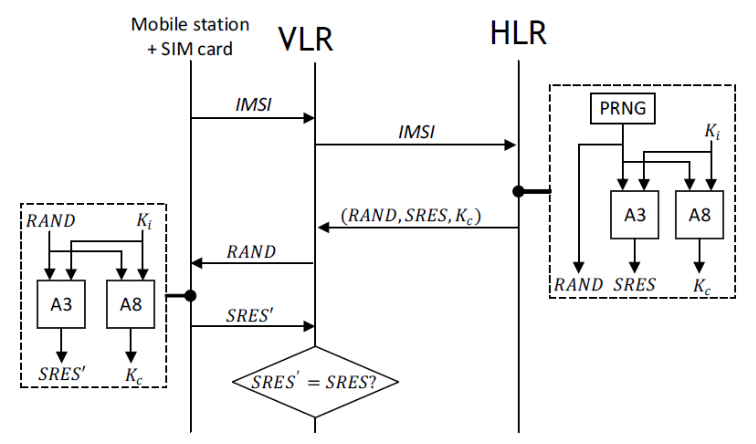
\includegraphics[width=0.7\textwidth]{images/GSM_auth.png}
    \end{solution}


    \question{4G networks - techniques used to enhance security}

    \question{GSM Authentication}

    \question{What is the primary purpose of rate adaptation in WiFi networks?}
    \begin{checkboxes}
        \choice To adjust the transmission power of devices based on network conditions.
        \choice To select the optimal data rate for transmitting data over the wireless channel based on the AP transmitter power.
        \choice To select the optimal data rate for transmitting data over the wireless channel based on the distance from the AP.
        \choice To adjust the transmission power of devices dynamically.
        \CorrectChoice None of the others.
    \end{checkboxes}

    \question{What is the primary purpose of handover in mobile networks?}
    \begin{checkboxes}
        \choice To encrypt voice and data transmissions for secure communication.
        \choice To seamslessy transfer an active call or data session from one mobile teriminal to another.
        \choice To manage billing and account information for mobile subscribers when they move between to Base Stations.
        \choice To increase the data transmission speed betwen mobile devices.
        \CorrectChoice None of the other options.
    \end{checkboxes}

    \question{What are the main components involved in the GSM authentication process?}
    \begin{checkboxes}
        \CorrectChoice SIM card, Authentication Center (AuC), and Home Location Register (HLR).
        \choice Mobile Equipment (ME), Visitor Location Register (VLR), and Base Transceiver Station (BTS).
        \choice Mobile Station (MS), Base Station Subsystem (BSS), and Network Switching Subsystem (NSS).
        \choice Mobile Management Entity (MME), Serving Gateway (SGW), and Packet Data Network Gateway (PGW).
        \choice None of the other options.
    \end{checkboxes}

    \question{Which of the following statements about PSK modulation is TRUE?}
    \begin{checkboxes}
        \choice Since each symbol has a different energy level, operating close to the saturation region of a power amplifier does not cause distortion, resulting in efficient use of the amplifier.
        \choice Since each symbol has a different energy level, operating close to the saturation region of a power amplifier causes distortion, resulting in a larger probability of error.
        \choice Since all the symbols have the same energy, operating close to the saturation region of a power amplifier causes distortion, resulting in a larger probability of error.
        \CorrectChoice Since all the symbols have the same energy, operating close to the saturation region of a power amplifier does not cause distortion, resulting in efficient use of the amplifier.
        \choice None of the other options.
    \end{checkboxes}


    \question{What are the advantages and disadvantages of having small or larger cells in mobile networks?}
    \begin{checkboxes}
        \choice Small cells are more expensive to deploy and maintain compared to larger cells, which are cheaper and more energy-efficient.
        \choice None of the other options.
        \choice Small cells are only suitable for urban areas, while larger cells can only be used in rural areas.
        \choice Small cells reduce interference and improve signal quality, whereas larger cells are prone to higher levels of interference and degraded signal quality.
        \CorrectChoice Small cells provide higher capacity and better coverage in dense areas but may require more frequent handovers as users move, while larger cells cover wider areas with fewer handovers but might have lower capacity in dense environments.
    \end{checkboxes}

    \question{Which of the following technologies are used in 4G networks to enhance security?}
    \begin{checkboxes}
        \CorrectChoice Advanced Encryption Standard (AES) for data encryption.
        \CorrectChoice Non-Access Stratum (NAS) security for signaling protection.
        \choice Implementation of advanced firewall technologies at the network core.
        \choice Temporary Mobile Subscriber Identity (TMSI) for user anonymity.
        \choice None of the other options.
    \end{checkboxes}

    \question{What is the difference between the IMSI and the TMSI in mobile networks?}
    \begin{checkboxes}
        \choice The IMSI identifies the mobile device, while the TMSI identifies the subscriber's location area.
        \choice The IMSI is a randomly generated number used for secure authentication, while the TMSI is a fixed identifier stored on the SIM card.
        \choice None of the other options.
        \CorrectChoice The IMSI is a unique identifier assigned to a mobile subscriber by the home network, while the TMSI is a temporary identifier used to protect the subscriber's identity during communications with the network.
        \choice The IMSI is used for billing and account management, while the TMSI is used for data encryption.
    \end{checkboxes}

    \question{How does the GSM network authenticate a subscriber using the SIM card?}
    \begin{checkboxes}
        \choice By requiring the subscriber to enter a personal identification number (PIN).
        \choice By sending a challenge (RAND) to the Authentication Center, which generates a response (SRES) using the Ki key.
        \choice By sending a challenge (RAND) to the SIM card, which generates a response (SRES) using the TMSI key.
        \choice By sending a challenge (RAND) to the SIM card, which generates a response (SRES) using the IMSI key.
        \CorrectChoice None of the other options.
    \end{checkboxes}


\end{questions}